\subsection{Panel operatora}
\label{lab:zad5}

Opracowany panel operatora

\ifdefined\CompileImages
    \begin{figure}[H]      
        \makebox[\textwidth][c]
        {
            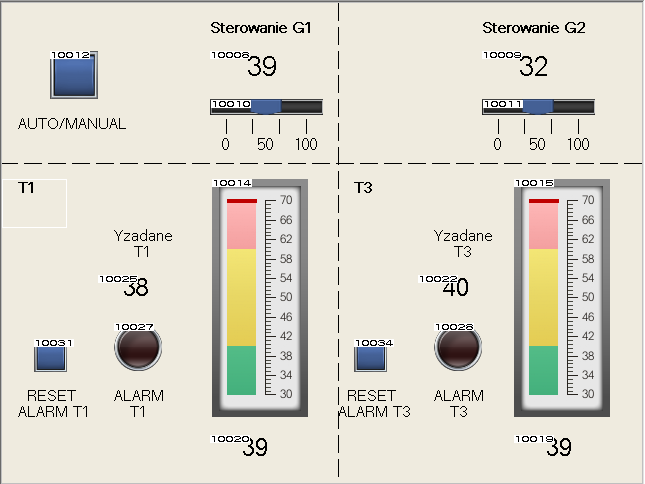
\includegraphics[width=5.2in,height=4.0in]{../lab/src/img/HMIStanowiskoGrzewczoChlodzace.png}
        }    
        \caption{Graficzny interfejs operatora stanowiska grzejąco-chłodzącego}
    \end{figure}
\fi


Operator może wybrać jeden z dwóch trybów automatyczny lub manualny poprzez naciśnięcie przycisku [AUTO/MANUAL].
W trybach tych wizualizowane mu są oraz możliwa jest modyfikacja wartości:
\begin{itemize}
    \item 
    Tryb manualny:
    \begin{itemize}
        \item Wartości wyświetlane nieedytowalne,
        \item Aktualna wartość temperatury na czujniku T1,
        \item Aktualna wartość temperatury na czujniku T3,
        \item Wartości wyświetlane edytowalne,
        \item Sterowanie grzałką G1,
        \item Sterowanie grzałką G2,
        \item Wartość zadana temperatury T1,
        \item Wartość zadana temperatury T3.
    \end{itemize}
    \item
    Tryb automatyczny:
    \begin{itemize}
        \item Wartości wyświetlane nieedytowalne,
        \item Aktualna wartość temperatury na czujniku T1,
        \item Aktualna wartość temperatury na czujniku T3,
        \item Sterowanie grzałką G1,
        \item Sterowanie grzałką G2,
        \item Wartości wyświetlane edytowalne,
        \item Wartość zadana temperatury T1,
        \item Wartość zadana temperatury T3.
    \end{itemize}
\end{itemize}


Dodatkowo zaimplementowany w zadaniu 2 mechanizm, 
który przy przekroczeniu temperatury \num{150.0} stopni Celsiusza wyłącza grzałkę sąsiadującą z czujnikiem, 
który zmierzył niebezpieczną temperaturę został wyposażony w diodę sygnalizującą o podanym stanie. 
Obok diody znajduje się przycisk, który resetuje alarm.

Założenia dotyczące wizualizacji:

HP HMI -  high performance human-machine interface - 
kierując się tym trendem wizualizacja procesu jest bardzo prosta, 
przekazuje tylko niezbędne informacje, a użyta paleta barw jest stonowana. 
\newline
Prawo Fittsa: Czas potrzebny do dojścia do celu jest funkcją wielkości celu i odległości do niego - 
dlatego też przycisk zmiany trybu pracy jest dość mały i znajduje się przy krawędzi ekranu użytkownika, 
aby nie pozwolić na nieprzemyślaną zmianę trybu sterowania.
\newline
Kluczowym parametrem dla użytkownika jest aktualna temperatura czujników T1 oraz T3, 
dlatego też został on przedstawiony nie tylko jako wyświetlana wartość, 
ale również jako wykres w kształcie walca. Rozwiązanie takie ma na celu ułatwienie odczytania tej wartości przez operatora nawet z dużych odległości.

\newpage
